\documentclass[UTF8]{ctexbeamer}	% Compile at least twice!
%\setbeamertemplate{navigation symbols}{}
\usetheme{Madrid}
% \setbeamertemplate{navigation symbols}{}
% \useinnertheme{rectangles}
% \useoutertheme{infolines}
% \useoutertheme[title,section,subsection=true]{smoothbars}
\useoutertheme{split}
\useinnertheme{rounded}
\setbeamertemplate{headline}{}
\usecolortheme{beaver}


% \usecolortheme{default}
% \usecolortheme{whale}
 
% -------------------
% Packages
% -------------------
\usepackage{
    amsmath,			% Math Environments
    amssymb,			% Extended Symbols
    enumerate,		    % Enumerate Environments
    graphicx,			% Include Images
    lastpage,			% Reference Lastpage
    multicol,			% Use Multi-columns
    multirow,			% Use Multi-rows
    pifont,			    % For Checkmarks
    stmaryrd,            % For brackets
    listings,
}
\usepackage[english]{babel}
\usepackage{graphicx}
\usepackage{animate}
\usepackage{xeCJK}
\usepackage{fontspec} 
\setCJKmainfont{gkai00mp.ttf}
% \usepackage{CJK}
% \lstset{language=C++}
% \lstset{extendedchars=false}
% \lstset{breaklines}


% -------------------
% Colors
% -------------------
% \definecolor{UniOrange}{RGB}{212,69,0}
% \definecolor{UniGray}{RGB}{62,61,60}
% \definecolor{UniRed}{HTML}{B31B1B}
% \definecolor{UniGray}{HTML}{222222}
% \setbeamercolor{title}{fg=UniGray}
% \setbeamercolor{frametitle}{fg=UniOrange}
% \setbeamercolor{structure}{fg=UniOrange}
% \setbeamercolor{section in head/foot}{bg=UniGray}
% \setbeamercolor{author in head/foot}{bg=UniGray}
% \setbeamercolor{date in head/foot}{fg=UniGray}
% \setbeamercolor{structure}{fg=UniOrange}
% \setbeamercolor{local structure}{fg=black}
% \beamersetuncovermixins{\opaqueness<1>{0}}{\opaqueness<2->{15}}


% -------------------
% Fonts & Layout
% -------------------
\usefonttheme{serif}
\usepackage{palatino}
\setbeamerfont{title like}{shape=\scshape}
\setbeamerfont{frametitle}{shape=\scshape}
\setbeamertemplate{itemize items}[circle]
% \setbeamertemplate{enumerate items}[default]


% -------------------
% Commands
% -------------------

% Special Characters
% \newcommand{\N}{\mathbb{N}}
% \newcommand{\Z}{\mathbb{Z}}
% \newcommand{\Q}{\mathbb{Q}}
% \newcommand{\R}{\mathbb{R}}
%\newcommand{\C}{\mathbb{C}}

% Math Operators
% \DeclareMathOperator{\im}{im}
% \DeclareMathOperator{\Span}{span}

% Special Commands
% \newcommand{\pf}{\noindent\emph{Proof. }}
% \newcommand{\ds}{\displaystyle}
% \newcommand{\defeq}{\stackrel{\text{def}}{=}}
% \newcommand{\ov}[1]{\overline{#1}}
% \newcommand{\ma}[1]{\stackrel{#1}{\longrightarrow}}
% \newcommand{\twomatrix}[4]{\begin{pmatrix} #1 & #2 \ #3 & #4 \end{pmatrix}}


% -------------------
% Tikz & PGF
% -------------------
\usepackage{tikz}
\usepackage{tikz-cd}
\usetikzlibrary{
    calc,
    decorations.pathmorphing,
    matrix,arrows,
    positioning,
    shapes.geometric
}
\usepackage{pgfplots}
\pgfplotsset{compat=newest}
\usepackage{wrapfig}
\usepackage{cite}


% -------------------
% Theorem Environments
% -------------------
\usepackage{amsthm}
\theoremstyle{plain}
\newtheorem{sit}{Situation}[section]
\newtheorem{prop}{Proposition}[section]
\newtheorem{rtm}{Theorem}[section]
\newtheorem{cor}{Corollary}[section]
\theoremstyle{definition}
\newtheorem{das}{Data structure}[section]
\newtheorem{nex}{Non-Example}[section]
\newtheorem{cla}{class}[section]
\newtheorem{emt}{}[section]
\newtheorem{defn}{Definition}[section]
\theoremstyle{remark}
\newtheorem{rem}{Remark}[section] 
\numberwithin{equation}{section}

\newcommand\caesura{$\mkern -8.5mu\raise -.2ex\hbox{\rotatebox[]{180}{\`}}\ $}

% -------------------
% Title Page
% -------------------
\title{\textcolor{red}{2022年硕博连读面试}}
%\subtitle{\textcolor{white}{Mathematics Conference for the Mysterious and dMagical}}  
\author{申请人: 谭焱 
% \newline \newline
%  \small{硕士导师: 王何宇\, \\
%  申请博士导师: 张庆海}
 }

\institute{\small{现硕士导师: 王何宇 \caesura 张庆海 \newline 拟转博士指导教师: 张庆海} \newline   \newline 浙江大学数学科学学院}
\date{\today} 


% -------------------
% Content
% -------------------
\begin{document}
% \begin{CJK}{GBK}{kai}

% Title Page
\begin{frame}
    \titlepage
\end{frame}


\begin{frame}
    \frametitle{提纲}
    \tableofcontents
\end{frame}

% Motivation
\section{个人基本情况介绍}


% \begin{frame}
%     \begin{emt}[过往受教育经历]
%         \begin{enumerate}
%             \item 高中在湖南师范大学附属中学就读时参与数学奥林匹克竞赛.
%         \end{enumerate}

%     \end{emt}
% \end{frame}


% Definitions & Examples
\begin{frame}[fragile]
    \frametitle{学习情况}
    \begin{enumerate}
        \item 研究生课程
              \begin{itemize}
                  \item 科研相关课程获得良好成绩
                        \begin{itemize}
                            \item 非线性问题的数学方法(92), 图形学的新进展(90) 等.
                        \end{itemize}
                  \item 英语阅读及写作方面
                        \begin{itemize}
                            \item 六级489分(阅读205)可以流畅阅读英文文献.
                            \item 通过研究生论文写作指导(92)打下坚实写作基础.
                        \end{itemize}
              \end{itemize}
        \item 科研训练
              \begin{itemize}
                  \item 系统地学习了代数拓扑和微分方程数值解的相关理论.
                  \item 锻炼了算法设计和编程实现能力.
                  \item 培养了将代数拓扑和微分方程数值解结合进行科学研究的思维方式.
              \end{itemize}
              % \item 编程学习
              % \begin{itemize}
              %     \item 熟悉Cpp14之前的大部分特性,使用Cpp完成张庆海老师多个项目.
              %     \item 流畅阅读Fortran, Python, Shell等语言的项目和使用make等工具.
              %     \item 独立AC LeetCode中200+道Hard题,能运用常见数据结构和高效算法.
              % \end{itemize}
    \end{enumerate}
\end{frame}

% \begin{frame}[fragile]
%    \frametitle{研究项目参与情况}
%     \small{\begin{enumerate}
%         \item 实现张庆海教授的论文(MATH COMP, 2020)中的二维空间上殷集的布尔代数.
%         % 为之后的三维空间内殷集之间的布尔代数的研究做好铺垫.
%         % 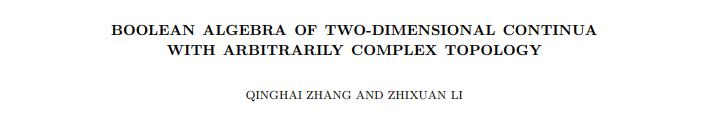
\includegraphics[width = \linewidth]{fig/articlename1.png}
%         % \item 和黎颖学长合作完成项目微地震反问题.最终得到一个能根据
%         % 检波器接收到的地震波信号输出合理的震源位置的程序.
%         \item 与邱云昊学弟分工推进三维殷集的表示,及编程实现在计算机上高效计算
%         三维殷集的布尔代数.
%         \item 独立尝试使用matlab在张庆海教授提出的CubicMARS方法追踪动边界
%         的过程中加入高精度追踪拓扑变化的时间点和发生位置.
%     \end{enumerate}}
% \end{frame}

\section{硕士阶段的科研工作}
\subsection{涉密的军工项目}
\begin{frame}
    \frametitle{涉密军工项目}
    \begin{itemize}
        \item 潜艇湍流尾迹的海洋表面特征等内波现象的研究, 用于潜艇追踪和隐身
              (\textcolor{red}{军科委基础加强重点项目}).
              \begin{figure}
                  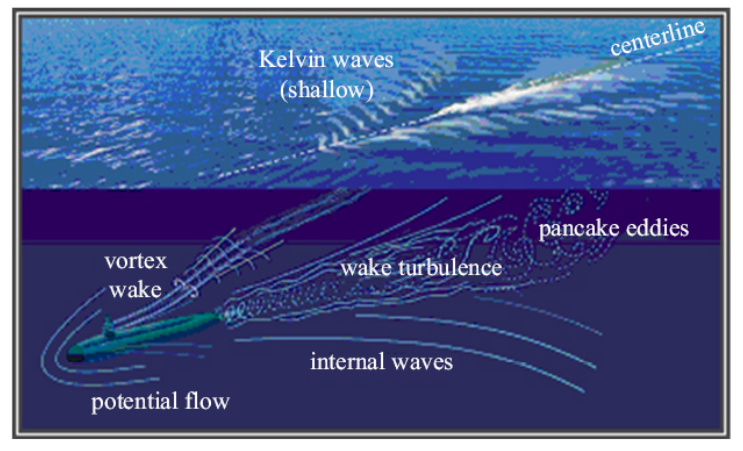
\includegraphics[width = 0.7\textwidth]{fig/s12.png}
                  \caption{水下潜艇产生的各种尾迹示意图, 包括开尔文尾迹, 内波, 湍流尾迹, 涡尾迹, 煎
                      饼旋涡.}
              \end{figure}
    \end{itemize}
\end{frame}

\subsection{\textcolor{red}{非涉密的三维殷集和布尔代数}}
\begin{frame}
    \frametitle{三维殷集的研究背景}
    \begin{itemize}
        \item 含有动边界的不可压流体在军工领域是非常重要的研究课题.
              % \item 流体建模相关研究少,数学模型和计算机算法都设计成避免在数值模拟时对流体
              % 进行几何建模.
              % \begin{enumerate}
              %     \item VOF方法中使用各个单元的体积分数重建边界.
              %     \item FT方法追踪边界上的示踪点,按顺序连接得到边界.
              %     \item LS方法求解隐式函数的边界.
              % \end{enumerate}
        \item 主流方法
        % (volume-of-fluids方法, front-tracking方法, level-set方法)的核心思想
        是对界面的几何和拓扑
              问题进行回避.
              \begin{enumerate}
                  \item 对等距变换的流场不能保证几何性质.
                  \item 对同胚映射的流场不能保证拓扑性质.
                  \item 精度最高为二阶精度.
                  \item 很难对拓扑变化进行严格的处理.
              \end{enumerate}
        \item 张庆海教授的思路是用\textcolor{red}{几何和拓扑的手段
                  研究几何和拓扑的问题},在二维空间中提出了殷集的定义(\textbf{MATH COMP, 2020}).
    \end{itemize}
    \begin{center}
        
\includegraphics[width = 0.9\textwidth]{fig/s14.png}
    \end{center}
\end{frame}


\begin{frame}
    \frametitle{三维殷集建模和实现布尔代数的意义}
    \begin{itemize}
        \item 三维殷集是军工项目的核心之一---对三维的动流相的建模.
        \item 是使用几何和拓扑的手段解决问题的奠基工作.
        \item 现有的``实体建模''与分析格格不入,无法追踪拓扑变化.
        \item 布尔代数是研究多相流流相拓扑的核心工具之一.
        \item 提供殷集的简单表示,可用于提高界面追踪的精度.
        \item 为处理拓扑变化提供了算法和理论支撑.
    \end{itemize}

    \begin{columns}
        \column{0.5\linewidth}<1->
        \centering
        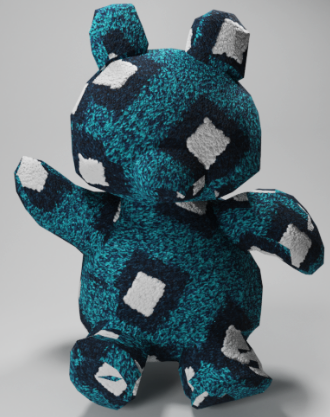
\includegraphics[width = .6\textwidth]{fig/s18.png}
        \column{0.5\linewidth}<1->
        \centering
        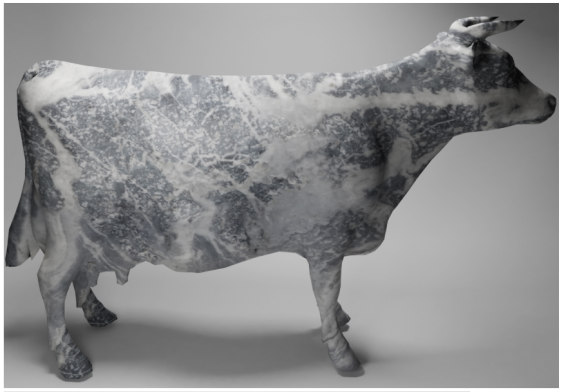
\includegraphics[width = .8\textwidth]{fig/s19.png}
    \end{columns}

    % \begin{itemize}
    %     \item 殷空间是一个跨领域的为有意义的物理区域恰当地建模的拓扑空间.
    %     \item 我们提供了殷集的简单表示方法,并且可以
    %     从殷集的表示方法中常数时间复杂度提取拓扑信息.
    %     \item 在殷空间上实现了高效的布尔代数,布尔代数是研究流相拓扑的核心工具之一.
    %     \item 为处理移动区域的拓扑变化提供了理论支持和程序接口.
    %     \item 与CubicMARS方法结合,可以提高界面追踪的精度,进而提高
    %     数值计算方法的精度.
    %     \end{itemize}
\end{frame}


\begin{frame}
    \frametitle{二维殷集}
    \begin{itemize}
        \item 二维空间中,任一个殷集可以唯一表示为
              \[\mathcal{Y} = \cup_j^{\bot \bot}\cap_i \text{int}(\gamma_{j, i} ),\]
              约当曲线 $\gamma_{j, i}$是$\mathcal{Y}$内第$j$个连通分量
              的第$i$条边界.
        \item 高效实现了殷集上的布尔代数.
              \begin{columns}
                  \column{0.3\linewidth}<1->
                  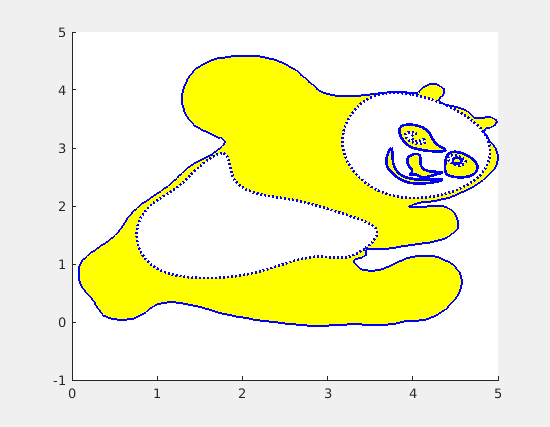
\includegraphics[width = \textwidth]{fig/p.png}
                  \column{0.3\linewidth}<1->
                  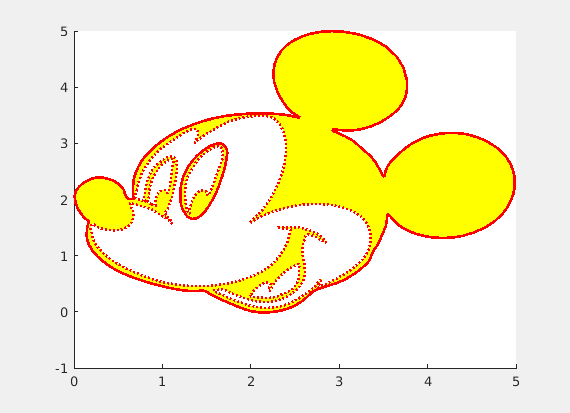
\includegraphics[width = \textwidth]{fig/m.png}
                  \column{0.3\linewidth}<1->
                  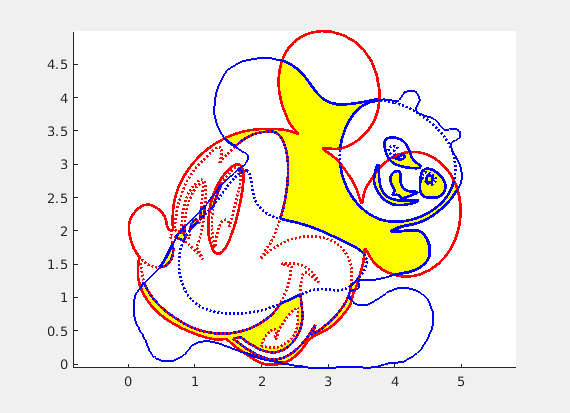
\includegraphics[width = \textwidth]{fig/pm.png}
              \end{columns}
              % \item 我编程实现了二维殷集的表示和布尔代数.
    \end{itemize}
\end{frame}

\begin{frame}
    \frametitle{黏合紧曲面}
    \begin{itemize}
        \item
              \textcolor{red}{二流形的分类定理} \newline
              有向的紧二流形是同胚于球或者圆环或它们的有限个的连通和.
              \begin{center}
                  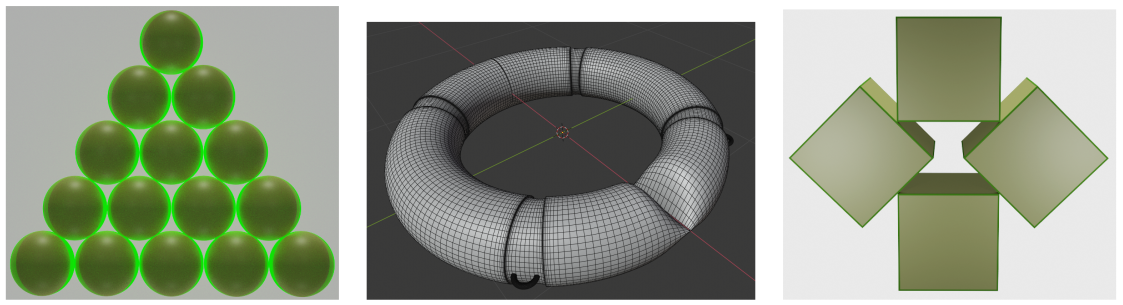
\includegraphics[width = .9\textwidth]{fig/s15.png}
              \end{center}


        \item 黏合紧曲面是一个二维连通紧流形或这种流形的一个商空间, 其商映射
              将多个与一维 CW 复形同胚的子集粘在一起; 将这个一维子集删除后
              该黏合紧曲面仍然是连通的.
    \end{itemize}
\end{frame}

\begin{frame}
    \frametitle{我的科研成果---三维殷集的数学模型及布尔代数}
    \begin{itemize}
        \item \textcolor{red}{三维殷集}:三维空间中边界有界的正则半解析开集.所有三维殷集构
              成的集合被称为殷空间,记为 $\mathbb{Y}$.
        \item 任一个殷集$\mathcal{Y} \in \mathbb{Y}$可以唯一表示为
              \[\mathcal{Y} = \cup_j^{\bot \bot} \cap_i \text{int}(\Gamma_{j, i}),\]
              黏合紧曲面$\Gamma_{j, i}$是$\mathcal{Y}$的第$j$个连通分量的第$i$个边界.
              % \item 黏合紧曲面是互相之间没有恰当交的闭合有向曲面.
    \end{itemize}
    \begin{columns}
        \column{0.5\linewidth}<1->
        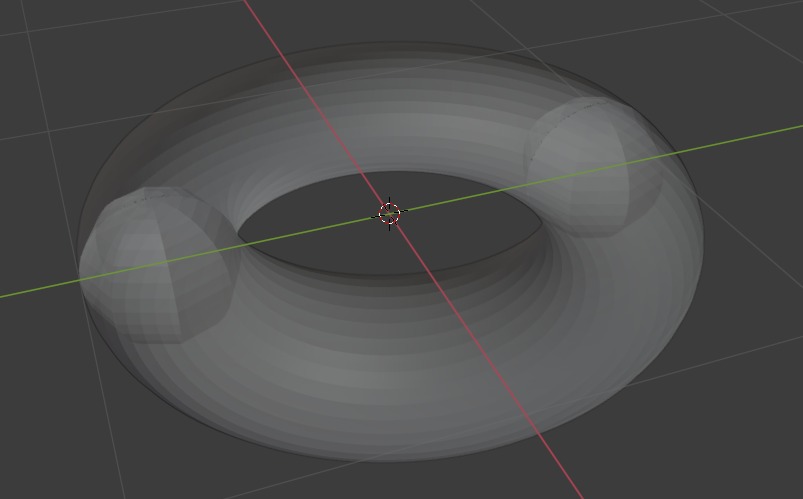
\includegraphics[width = \textwidth]{fig/s1.png}
        \column{0.5\linewidth}<1->
        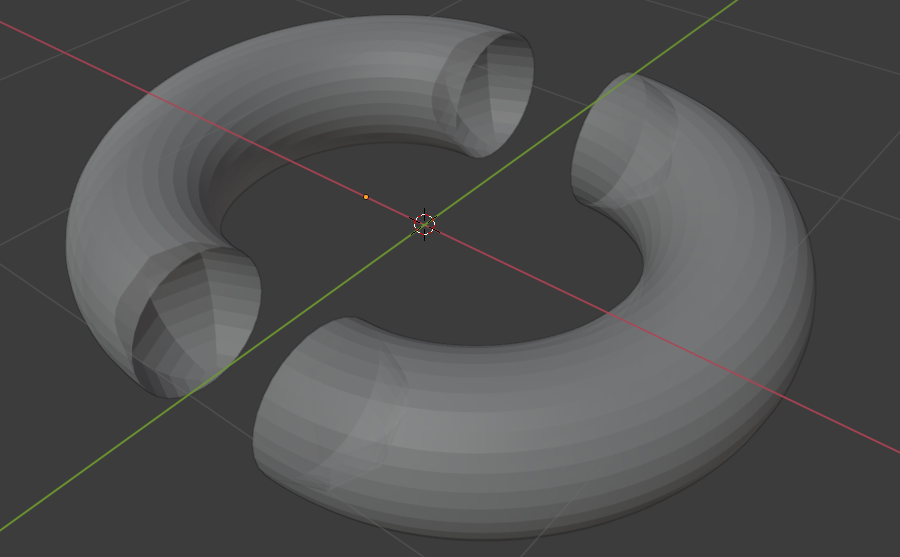
\includegraphics[width = \textwidth]{fig/s2.png}
    \end{columns}
\end{frame}

\begin{frame}
    \frametitle{布尔代数实现方式}
    \begin{enumerate}
        \item 计算殷集边界上的所有非流形点.
        \item 沿非流形点剪开黏合紧曲面得到若干曲面片.
        \item 根据交并补的需要删除曲面片或改变曲面片方向.
        \item 将曲面片重新黏合成黏合紧曲面集合.
        \item 黏合紧曲面集合唯一表示一个三维殷集作为布尔运算结果.
    \end{enumerate}
    \begin{columns}
        \column{0.4\linewidth}<1->
        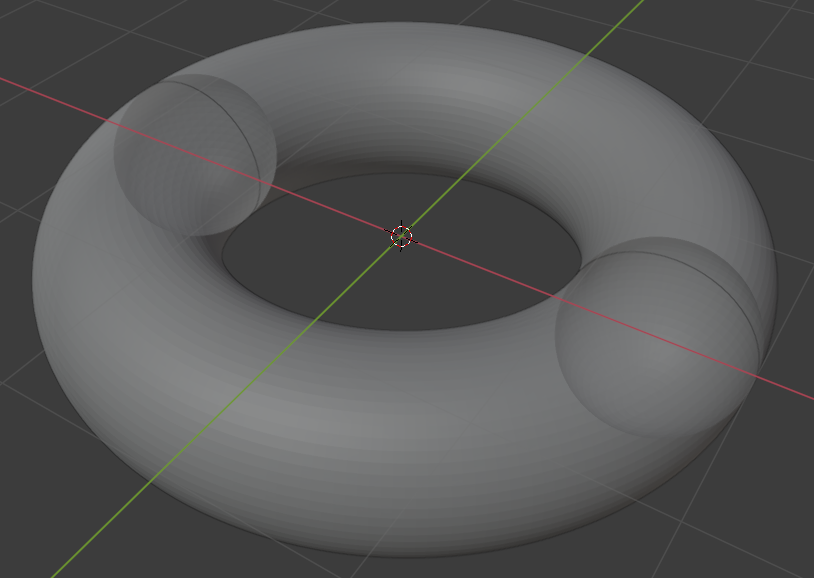
\includegraphics[width = \textwidth]{fig/s3.png}
        \column{0.4\linewidth}<1->
        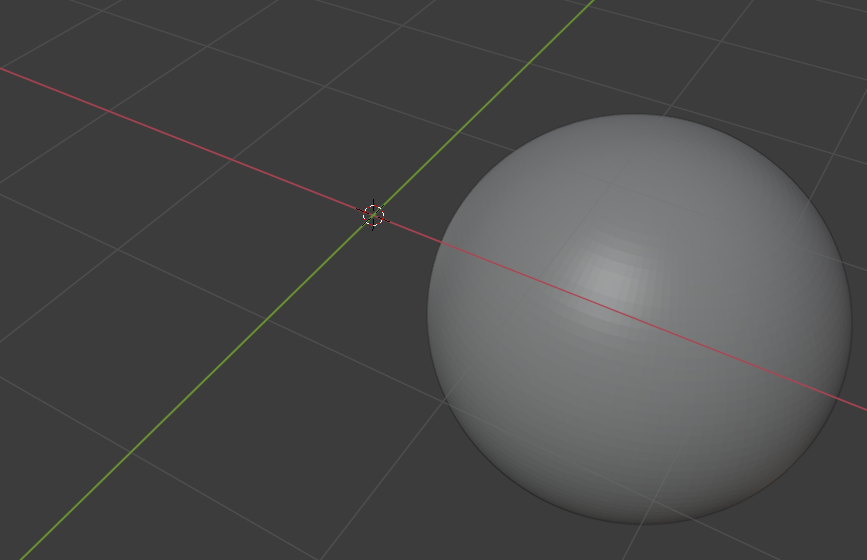
\includegraphics[width = \textwidth]{fig/s4.png}
    \end{columns}
\end{frame}

\begin{frame}
    \frametitle{布尔代数结果图}
    \begin{itemize}
        \item 沿非流形点剪开黏合紧曲面得到曲面片集合
              \begin{columns}
                  \column{0.4\linewidth}<1->
                  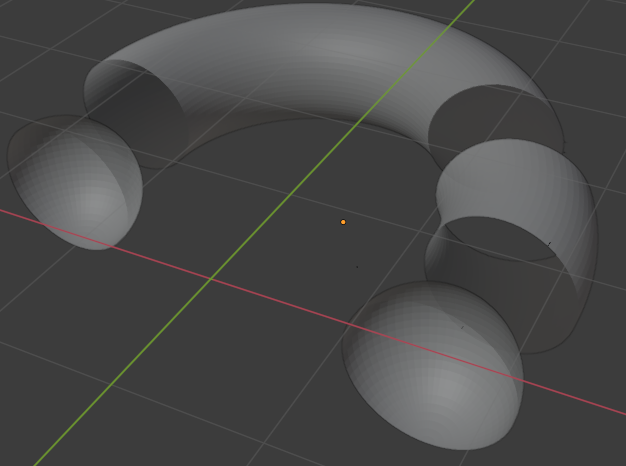
\includegraphics[width = \textwidth]{fig/s16.png}
                  \column{0.4\linewidth}<1->
                  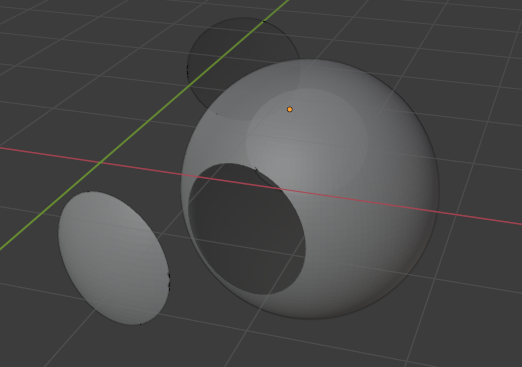
\includegraphics[width = \textwidth]{fig/s17.png}
              \end{columns}
        \item 交
              \begin{columns}
                  \column{0.4\linewidth}<1->
                  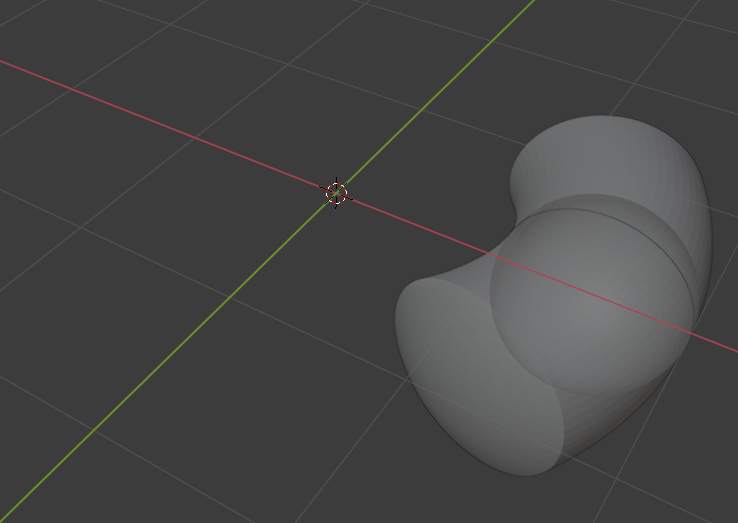
\includegraphics[width = \textwidth]{fig/s5.png}
                  \column{0.4\linewidth}<1->
                  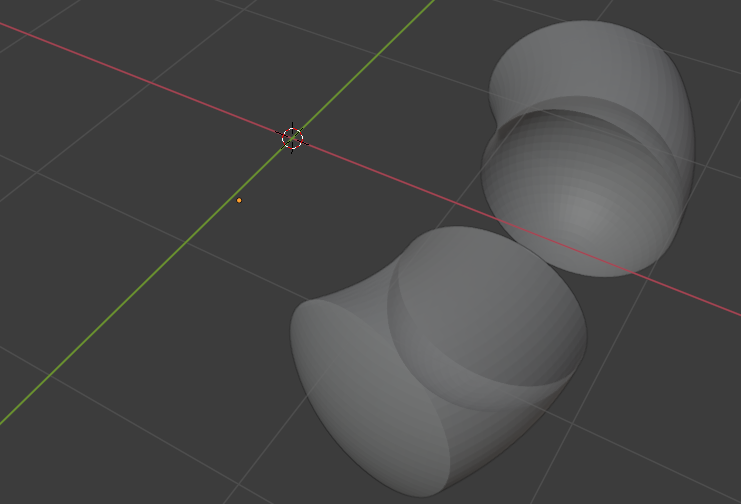
\includegraphics[width = \textwidth]{fig/s6.png}
              \end{columns}
    \end{itemize}
\end{frame}

\begin{frame}
    \begin{itemize}
        \item 并 \begin{columns}
                  \column{0.4\linewidth}<1->
                  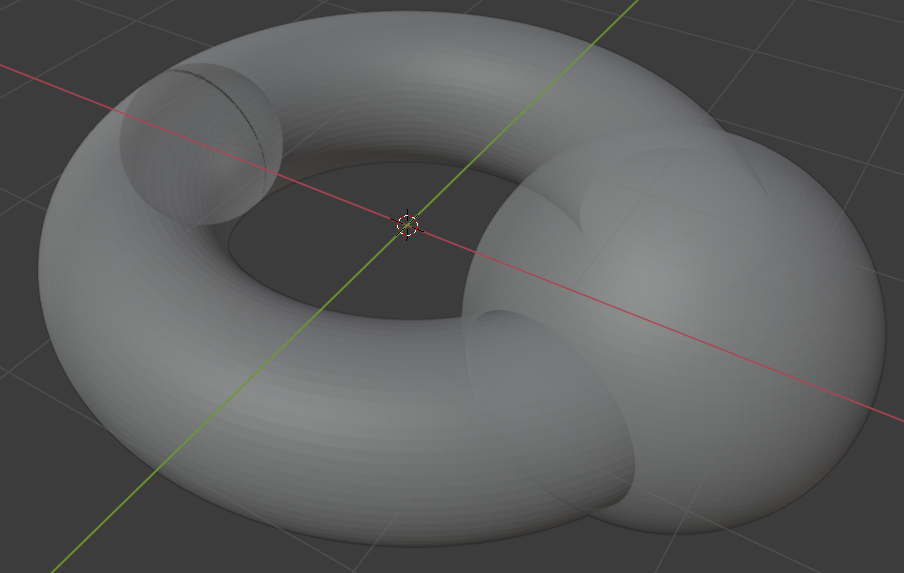
\includegraphics[width = \textwidth]{fig/s7.png}
                  \column{0.4\linewidth}<1->
                  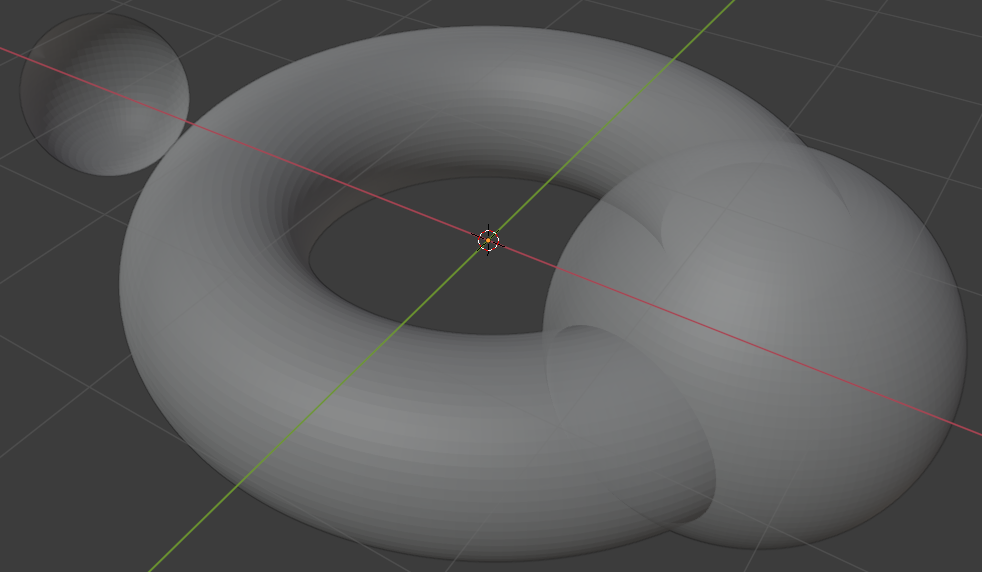
\includegraphics[width = \textwidth]{fig/s8.png}
              \end{columns}
        \item 复杂几何结构
              \begin{columns}
                  \column{0.3\linewidth}<1->
                  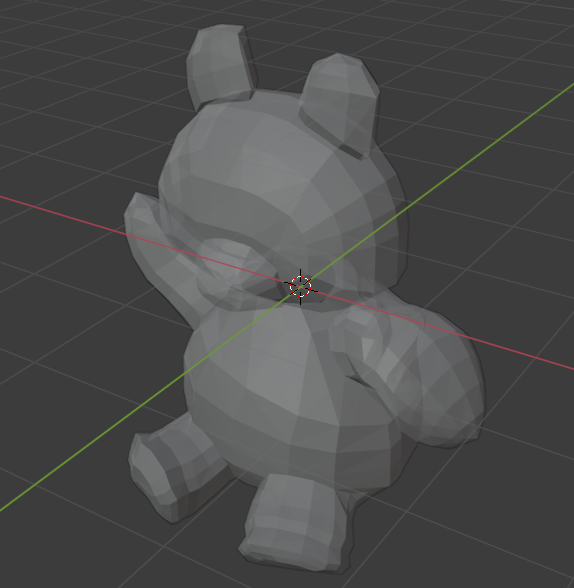
\includegraphics[width = \textwidth]{fig/s10.png}
                  \column{0.3\linewidth}<1->
                  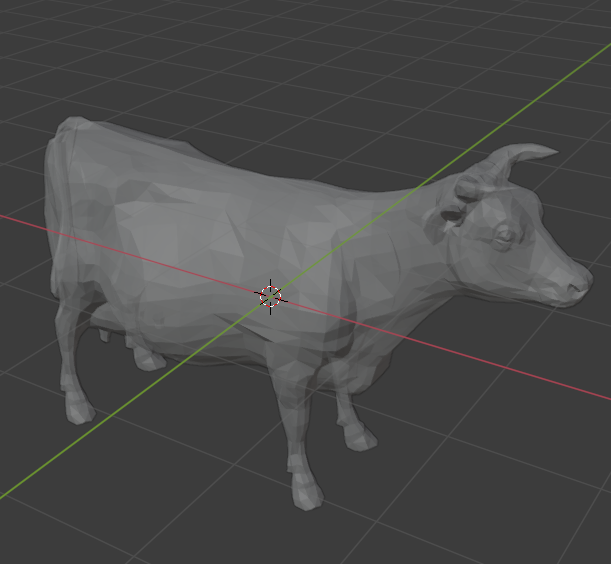
\includegraphics[width = \textwidth]{fig/s9.png}
                  \column{0.3\linewidth}<1->
                  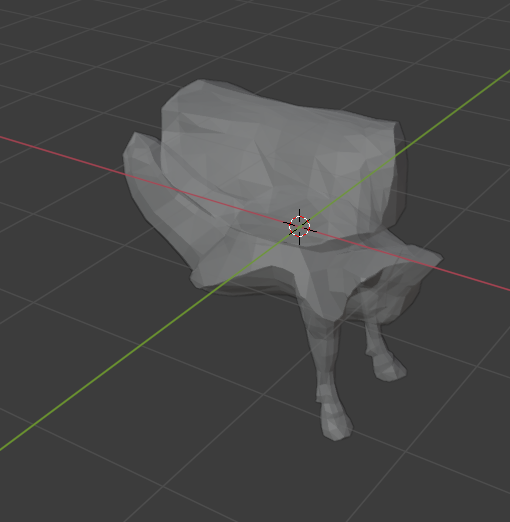
\includegraphics[width = \textwidth]{fig/s11.png}
              \end{columns}
    \end{itemize}
\end{frame}

\begin{frame}
    \frametitle{论文在投}
    \centering
    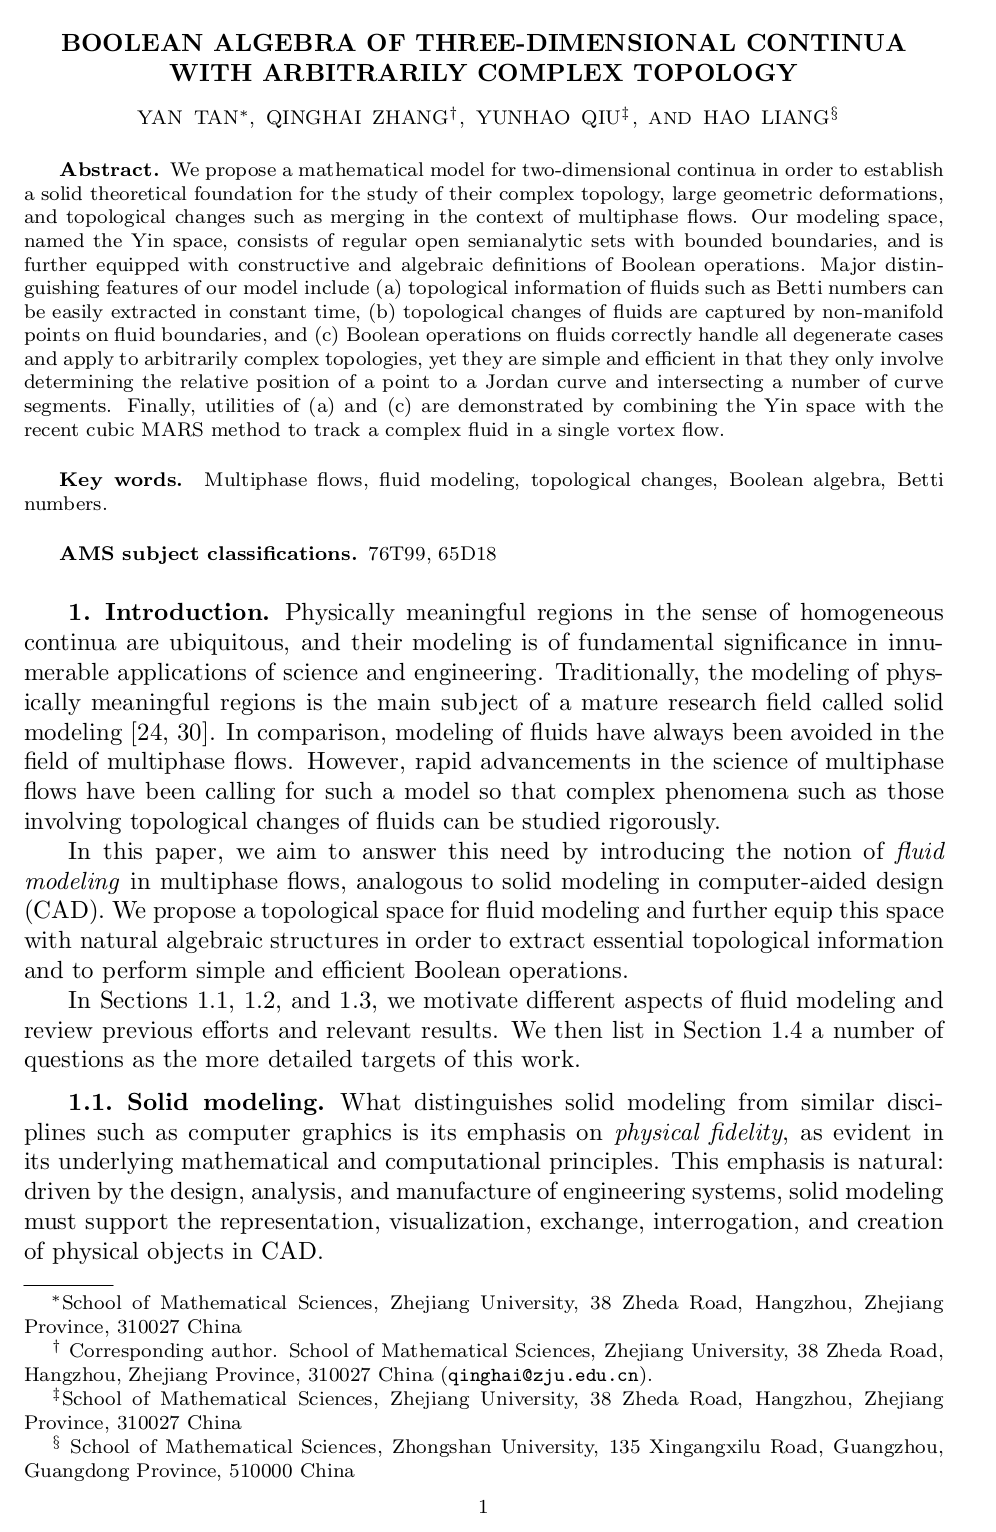
\includegraphics[height = \textheight]{fig/SIAM_Review.png}
\end{frame}

% \subsection{CubicMARS方法追踪拓扑变化}
% \begin{frame}
%     \frametitle{研究背景}
%     \begin{itemize}
%         \item 多相流的研究在军事国防,医学仿生,核能工业,海洋工程,国民经济等许多重大
%         领域中都占有举足轻重的地位; 而界面追踪问题是多相流数值计算中最基本的子问题之一.
%         % 其重要性体现在
%         % \begin{enumerate}
%         %     \item 界面追踪不可避免的影响到流相计算精度.
%         %     \item 在表面张力不可忽略的多相流问题中,界面追踪准确性低会导致数值模拟
%         %     结果脱离物理实际.
%         % \end{enumerate}
%         \item 现有的界面追踪方法在过去都取得了巨大成功,但是随着多相流研究
%         的进展,这些方法逐渐捉襟见肘.
%         \begin{enumerate}
%             \item 现有的方法计算精度不够高.
%             \item 在处理流相拓扑结构变化时随意性大.
%             \item 现有的显式界面追踪方法缺乏严格的系统理论支持.
%         \end{enumerate}
%         \item 张庆海教授18年提出的CubicMARS方法是一套用于对界面追踪问题的分析
%         的普适理论,
%         是时空一致四阶以上精度的界面追踪方法.
%     \end{itemize}

% \end{frame}

% \begin{frame}
%     \frametitle{研究的方向} 
%     \begin{itemize}
%         \item 在CubicMARS方法的基础上,结合二维殷集,增添对拓扑变化的处理.
%         \item 需要在有拓扑变化的流相追踪过程中保持计算精度.
%         \item 期望同样能高精度捕捉流相拓扑变化的时间点和位置.
%     \end{itemize}
%     \centering
%     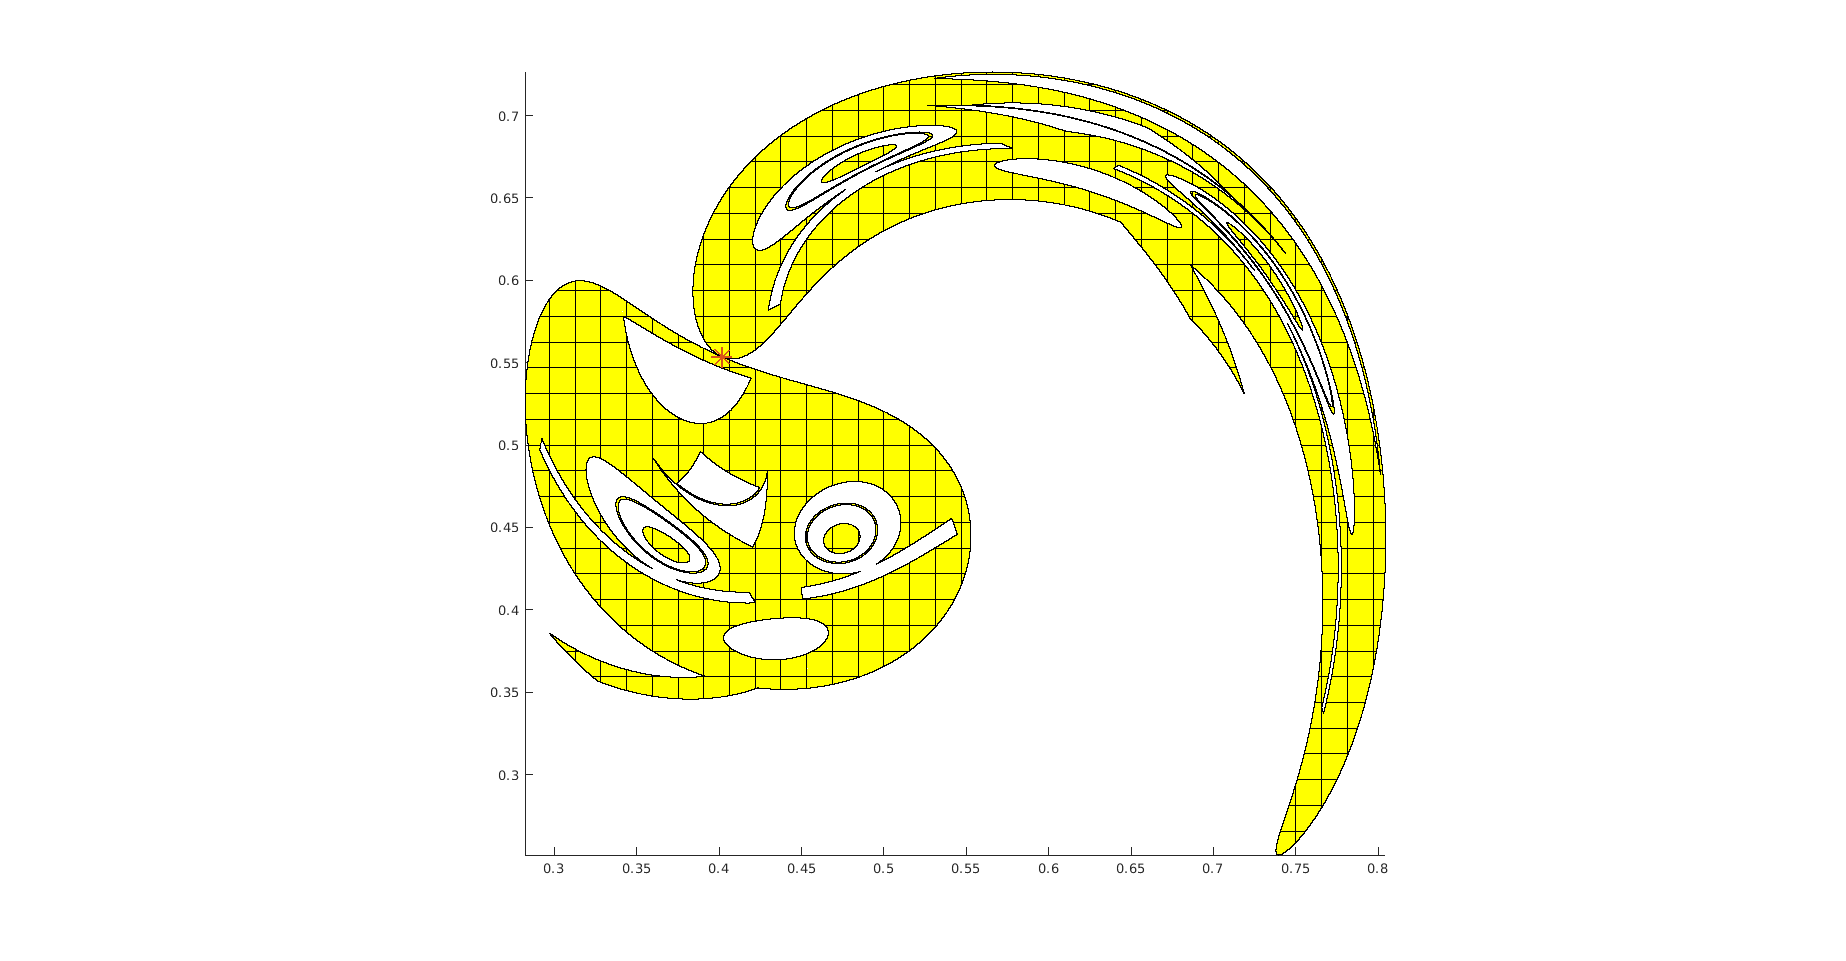
\includegraphics[width = 0.7\textwidth]{fig/s13.png}
% \end{frame}

\section{博士阶段的研究计划}
\subsection{流相的拓扑变化}
\begin{frame}
    \frametitle{博士研究计划}
    \begin{center}
        % \includegraphics[width = 0.7\textwidth]{fig/fig/Mars.gif};
        \animategraphics[autoplay,
            loop,
            width=.5\textwidth]{5}{fig/gif/1/vortex80N64step00}{0}{62}
    \end{center}
    \begin{itemize}
        \item 现有方法不能精确捕捉和刻画拓扑变化.
        \item 结合殷集对流体建模,在张庆海教授(SIAM J SCI COMP, 2018)
              提出的CubicMARS方法上
              新增对拓扑变化的处理,并且高精度捕捉拓扑变化的时间点和位置.
        \item 这个研究是三维殷集在军工项目中的重要应用,是项目的核心部分.
    \end{itemize}
\end{frame}



\section*{}
\begin{frame}
    \centering\huge
    \textcolor{red}{请各位老师批评指正!}
\end{frame}
% \end{CJK}
\end{document}